%\documentclass[a4paper,11pt]{article}
%\usepackage{graphicx}
%\usepackage{mathrsfs}
%\usepackage{amssymb,amsfonts,amsmath}
%\usepackage{multirow}
%\usepackage{epsfig}
%\usepackage{subfigure}
%
%\def\pdfshellescape{1}
%\usepackage{epstopdf}
%
%\usepackage{color}
%\usepackage{float}
\documentclass[11pt,a4paper,oneside]{article}

% packages
\usepackage[top=25.4mm,bottom=25.4mm,left=31.8mm,right=31.8mm]{geometry}
\usepackage{fancyvrb}   % fancy verbatim
\usepackage{enumerate}  % extra styles for enumerate list environment
\usepackage{setspace}   % setting paragraph spacing
\usepackage{array}      % text wrap in table cell, \multicolumn
\usepackage{multirow}   % \multirow
\usepackage{graphicx}
\usepackage{amsmath}    % using split env, cooperating with ntheorem package
\usepackage[amsmath,amsthm,thmmarks]{ntheorem}
\usepackage[urw-garamond]{mathdesign}
\usepackage[T1]{fontenc}
\newtheorem{thm}{Theorem}[subsection]  % SECTION_NUM.THEOREM_NUM
\newtheorem{cor}[thm]{Corollary}
\newtheorem{lem}[thm]{Lemma}           % SECTION_NUM.LEMMA_NUM
\numberwithin{figure}{section}


\begin{document}

\title{Assignment 1}
\author{Institute of Computing Technology, \\
        Chinese Academy of Sciences, Beijing, China }
\date{\today}
\maketitle

\noindent
\textbf{Notice}
\begin{enumerate}
\item Due date
      \begin{itemize}
      \item Oct. 26, 2012 for CS711008Z.
      \item Nov. 7, 2012 for CS6012.
      \end{itemize}
\item Please send your answer in hard copy.
\item You can choose one problem from Problem 1-2, and one problem from Problem 3-4.
\item When you're asked to give an algorithm, you should do at least the following things:
      \begin{itemize}
      \item Describe your algorithm in words or pseudo-code;
      \item Prove that your algorithm can give the right answer;
      \item Analyse the complexity of your algorithm.
      \end{itemize}
\item You can present your answer in English or in Chinese.
\end{enumerate}

\section{Stable Matching}
\noindent
Decide whether you think the following statement is true or false. 
If it is true, give a short explanation. 
If it is false, give a counterexample.
\\ \\
\textit{True or false?} Consider an instance of the Stable Matching Problem 
in which there exits a man $m$ and a woman $w$ such that 
$m$ is ranked first on the preference list of $w$ and $w$ is ranked first on the preference list of $m$. 
Then in every stable matching $S$ for this instance, 
the pair $(m, w)$ belongs to $S$.
%
%
\section{Stable Matching}
\noindent
In the \textit{Gale-Shapley} algorithm of the Stable Matching Problem,
an unmarried man proposes to his highest-ranked woman to whom he has not yet proposed, 
woman never proposes to man, and the algorithm yields the stable matching $S^*$.
Now, suppose an unmarried \textit{woman} proposes to her highest-ranked man 
to whom she has not yet proposed, \textit{man} never proposes to woman, 
and the algorithm yields the stable matching $S^*$'.
\\ \\
\textit{True or false?} For \textit{every} instance of the Stable Matching Problem, $S^* = S^*$'.
\\ \\
Write a program to implement the above two algorithms in your favorite language,
and give your answer based-on your implementation.
%
%
\section{Complexity Analysis}
\noindent
A sequence of $n$ operations is performed on a data structure.
The $i$th operation costs $i$ if $i$ is an exact power of $2$, and $1$ otherwise.
Use a \textit{potential method} to determine the amortized cost per operation.
%
%
\section{Complexity Analysis}
In stock market, HH-index(historically highest) of the current price is $k$ means that 
current price is the highest price in the previous $k$ days, 
but not the highest one in the previous $k+1$ days. 

For example, the price changes as shown in the following figure. 
%
\begin{figure}[htbp]
\centering
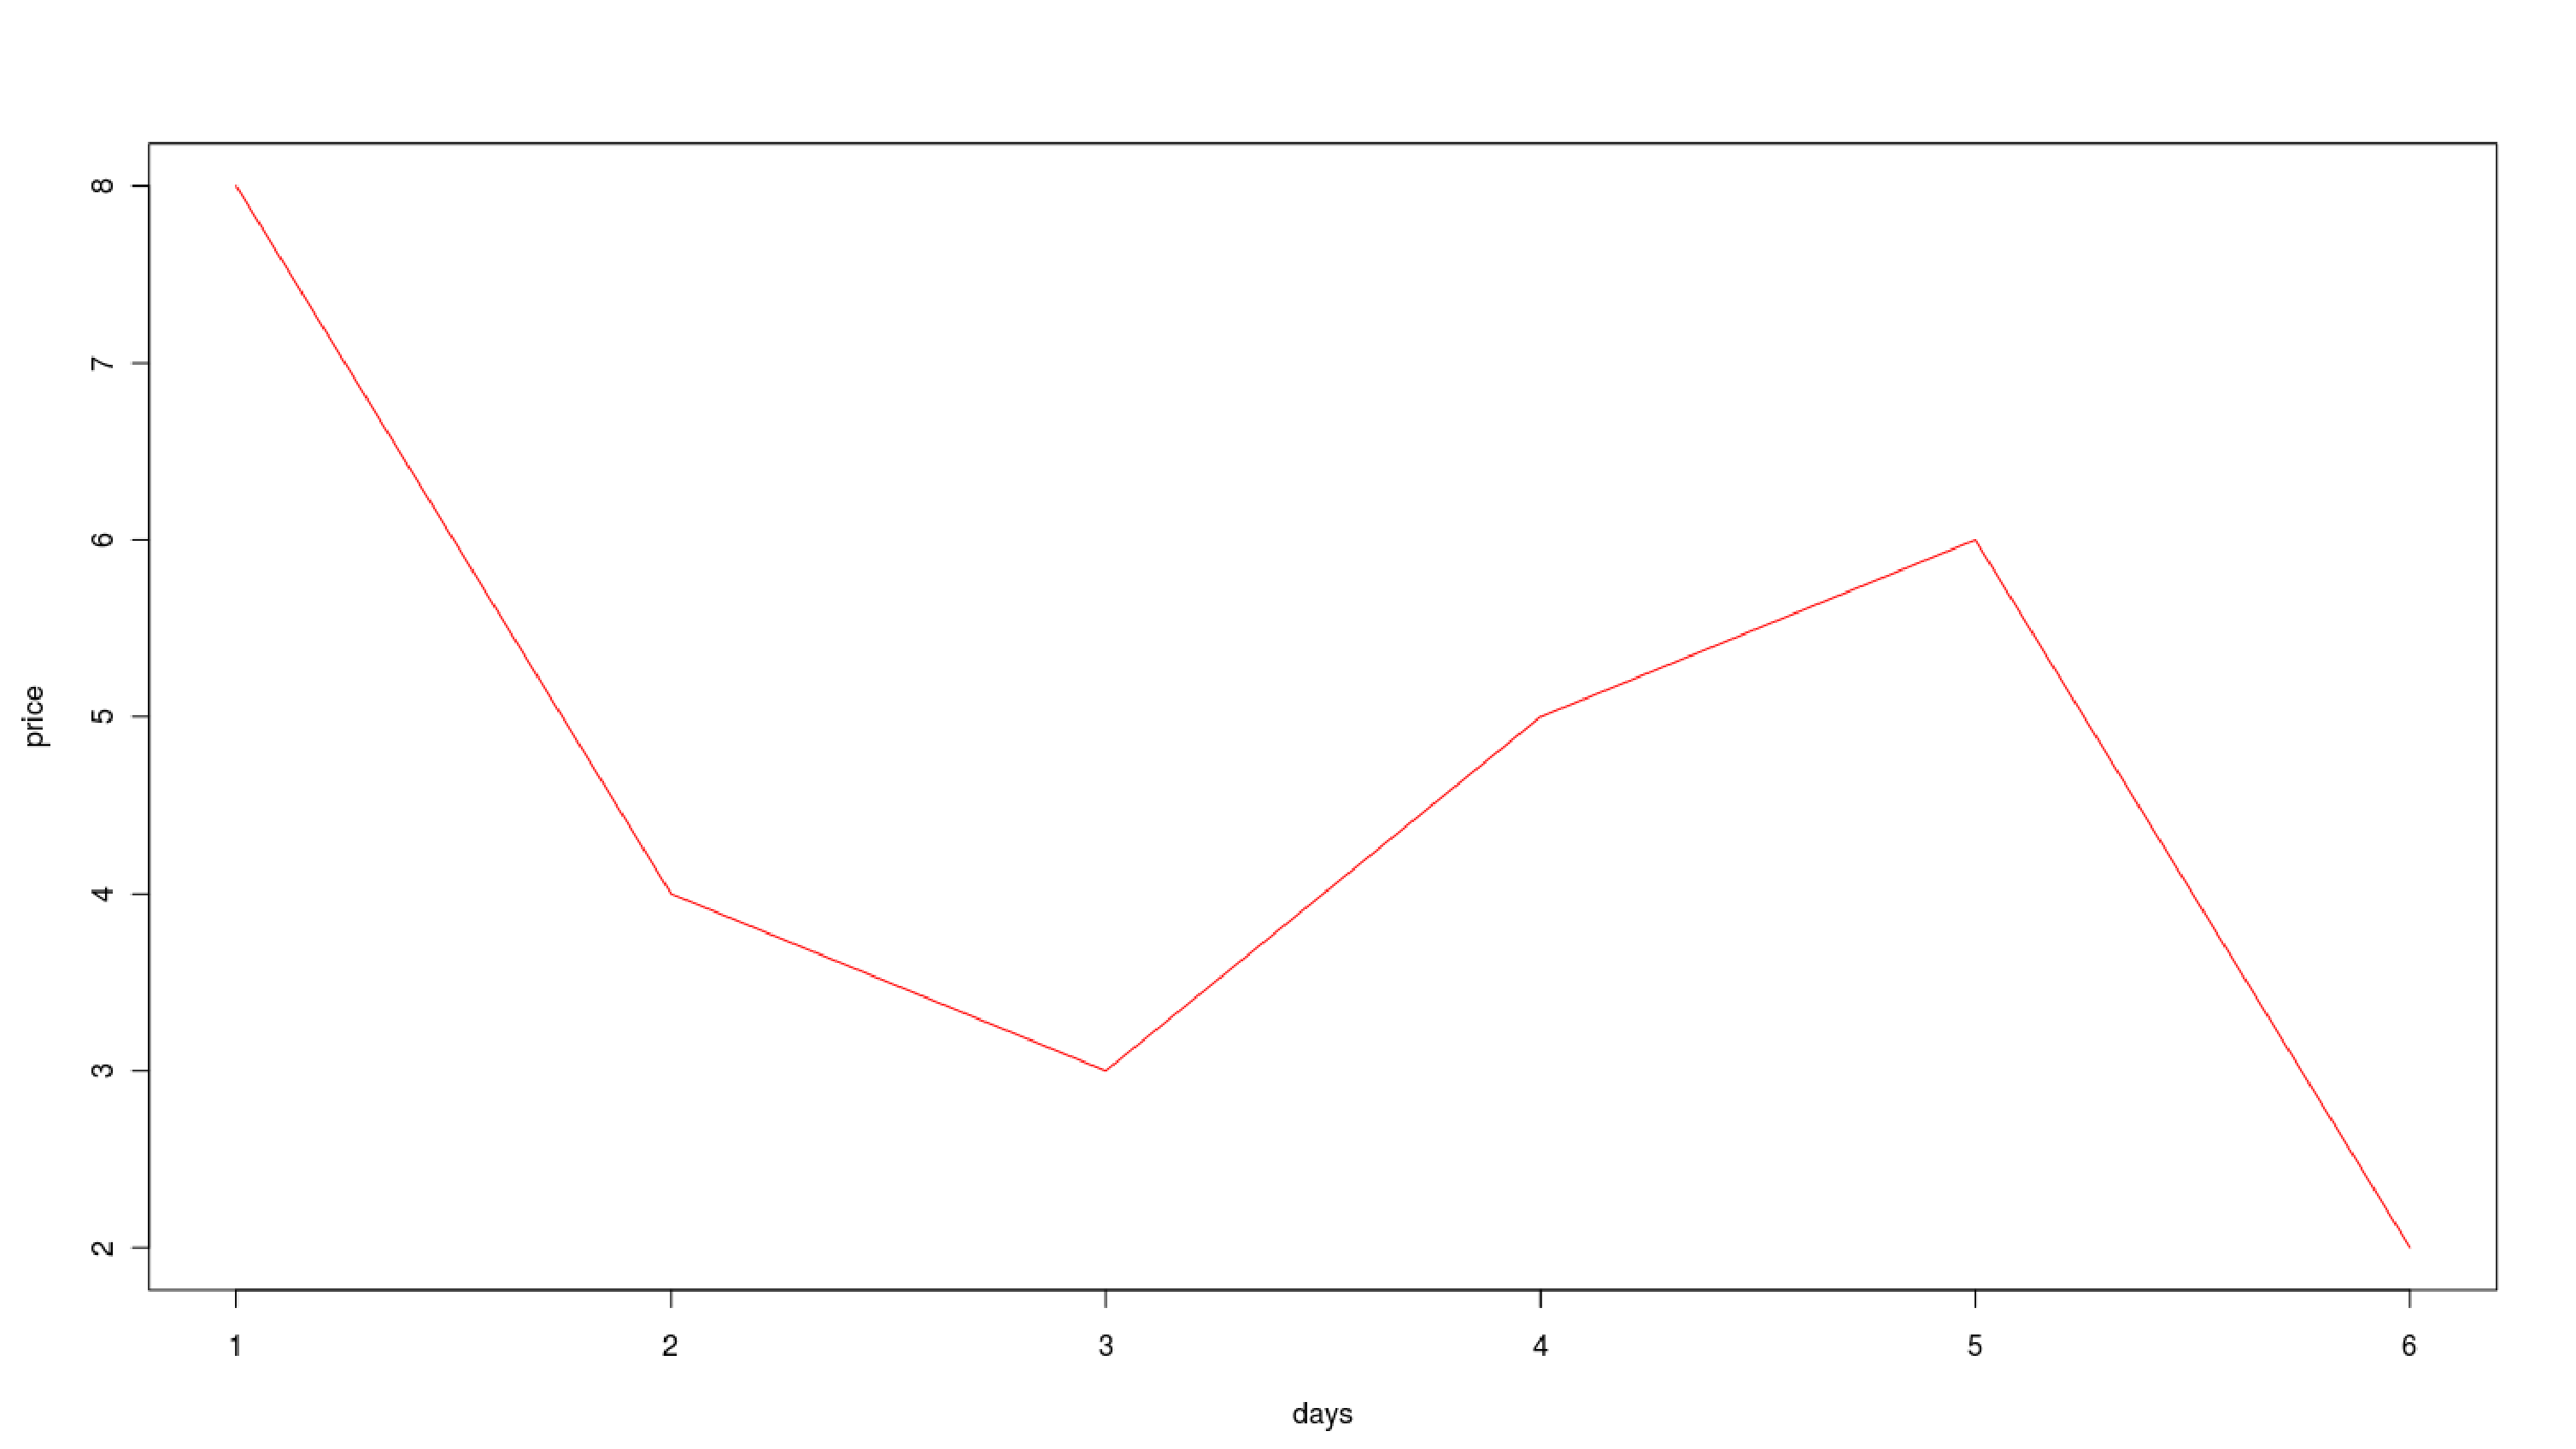
\includegraphics[width = 6in]{price.eps}
\label{fig:prices}
\end{figure}
%
\\
The price in Day $5$ is the highest in Days $5, 4, 3, 2$,  
but not highest one in Days $5, 4, 3, 2, 1$, thus $HH(5) = 4$;
\\
The price in Day $4$ is the highest in Days $4, 3, 2$,  
but not highest one in Days $4, 3, 2, 1$, thus $HH(4) = 3$;
\\
The price in Day $3$ is the highest in Day $3$,  
but not highest one in Days $3, 2$, thus $HH(3) = 1$;
\\
The input in this example is $8, 4, 3, 5, 6, 2$, 
the answer is $1, 1, 1, 3, 4, 1$.
\\ \\
Given the prices of $n$ days, 
please give an algorithm of $O(n)$ time complexity to calculate the HH-index of all days.

\end{document}
